\part{Vermischtes}
\setcounter{section}{0}

\section{Trigonometrie}
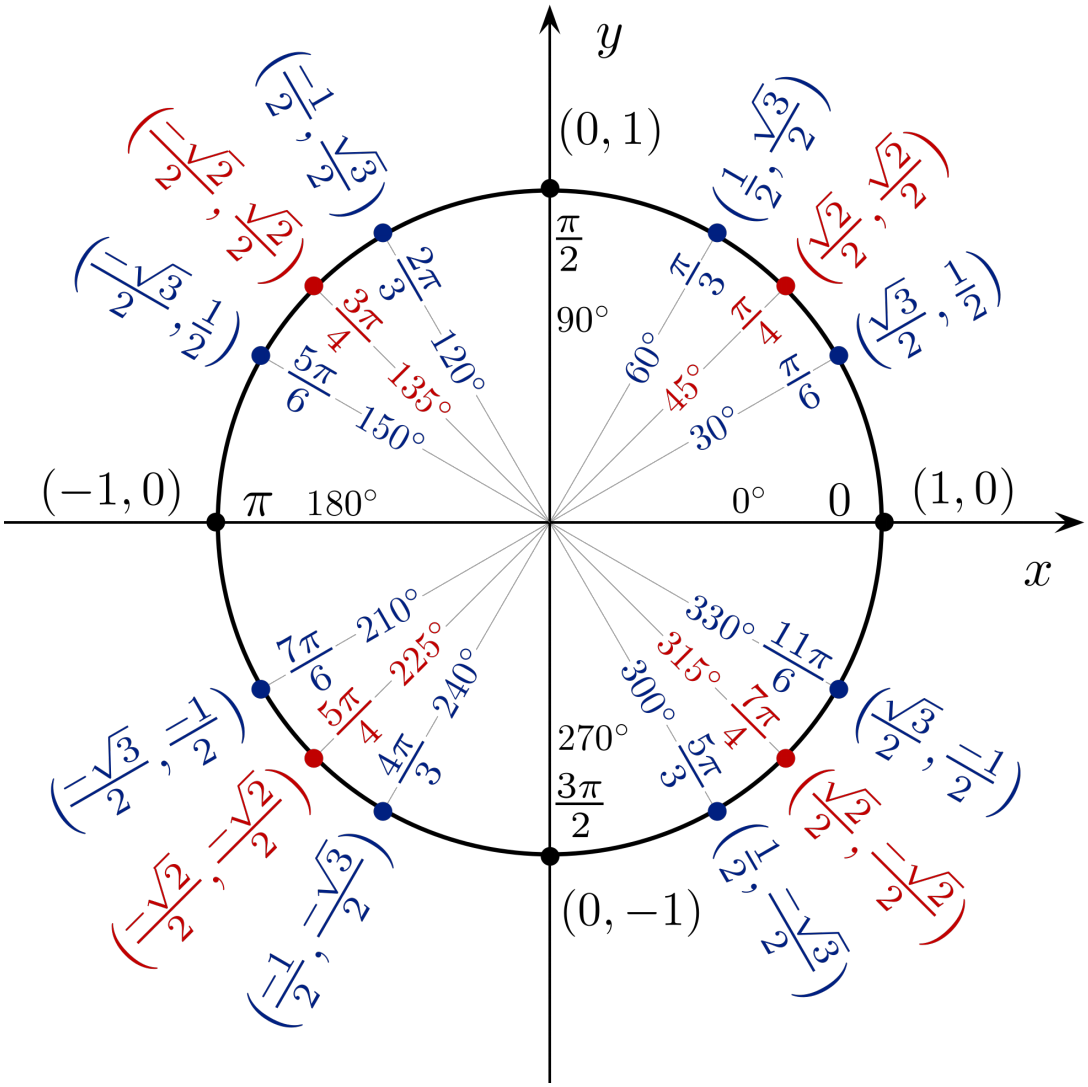
\includegraphics[scale=0.225]{sinus_cosinus}

\section{Quadratic Formula}
\[ x = \frac{-b + \pm \sqrt{b^2 - 4 a c} }{2 a} \]

\section{Proofs}
\Beweis[$\sin(x) < x$] Case distinction $\rightarrow$ Mean-Value-Theorem \\

\Beweis[Fixpunkt 6.4a] Case distinction $\rightarrow$ Mean-Value-Theorem \\

\Beweis[$1+x \leq e^x \leq 1/(1-x)$] Case distinction $\rightarrow$ Mean-Value-Theorem

\section{Am Schluss}
\begin{itemize}
	\item 'c' nirgends vergessen?
\end{itemize}